\section{Discussion}
\label{sec:discussion}

\subsection{Simulations show quadcopter limitations when attempting extreme maneuvers at full speed}
\fref{fig:onefifthspeed}--\fref{fig:onetwentiethspeed} show that as the speed was reduced, the quadrotor was able to more closely follow the desired hummingbird trajectory. A look at the RMSE calculations in \fref{tab:RMSE} and \fref{tab:icRMSE} shows that this was indeed the case. The quadrotor was unable to obtain an RMSE (the mean distance error value) of less than one meter before gain tuning, even when flying at one twentieth the hummingbird's true speed. At this slower speed, the error is still exorbitantly high at a value ten times greater than my definition of a successful trajectory flight, and showed a standard deviation that was more than five times my defined value for a successful flight. After gain tuning, small improvements were made to the overall reduction of the RMSE value at each trial; however, they were still several times higher than I had defined for a successful trajectory flight. Although control gain optimization may lead to a successful trial at slower speeds, several changes will likely need to be made to the structure of the controller in order to obtain desireable results at the higher speed trials. This simulation assumes a linearization region about the ``hover'' state, which doesn't lead it well to controlling the quadrotor accurately through this extreme maneuver.

%AFTERTHOUGHTS: If I am able to accomplish a working simulation with the Anna’s Hummingbird courtship dive maneuver, I will try to make the simulation slightly more general so it can apply to a wide variety of hummingbird dives and maneuvers. This can include evasive maneuvers, and potentially other types of stunts.

The results suggest limits to path planning algorithms, which often treat lower level platform dynamics as a black box that ought simply perform as advertised. At low advance speeds, the low level onboard flight controller in auto level mode is able to deliver controlled positions at the rate commanded by the higher level path planning algorithm. As speed increases, however, rates become important and at some point the flight controller is not longer able to assume a series of quasi-steady positions as dictated by the higher level path planning algorithm. My advisor suggested coining the term for this as ``The Marcello Limit''; in human quadrotor pilots this is the point at which they transition to flying ``in acro'' (e.g. control of angular rates rather than control of position and angular position). In future projects, it would be advisable to develop mathematical foundations for predicting the Marcello Limit, and to consider alternate control strategies (i.e. an autonomus variant of \lstinline{ACRO} mode) to use at the higher approach speeds. 




\subsection{Improved control in simulation}
The purpose of improving the controller given by the simulation was to find a way to reduce the root mean square error between the desired trajectory path and the actual trajectory path flown by the quadrotor. Several attempts were made at error reductions, with limited success. The changes that I made to the control gains did improve the system, and the results of the marginal analysis even suggested that it could be enhanced further; however, this controller is simply not sufficient for executing the extreme maneuvers outlined in this report. The main issue with the current controller is that it only takes into account one timestep at a time and iteratively makes adjustments based off of each new incoming position command. In this way, it fails to anticipate the necessity of large acceleration requirements (namely at the top of the dive when the hummingbird is diving downward, and bottom of the dive when the hummingbird pulls 9g to soar up out of the dive \cite{clark2009courtship} to properly pull the quadcopter out of the dive and follow the hummingbird trajectory. As such, a completely new controller would need to be outfitted on the simulation in order to get the results that I desire.




\subsection{Experimental flight demonstration next steps}
When the global COVID-19 pandemic is over, the next step to the autonomous experimental demonstration will involve the conversion of the controller code used in the \MATLAB\ simulation to something that can be used on the Crazyflie hardware. The controller will therefore be written in Python, as it is similar to \MATLAB\ and can be used on the Crazyflie with the ROS package. The other option would be to use C programming language, but since the ROS demo I'm using is in Python it would be wiser to stay consistent with that language for the hardware. Therefore Python will be used to implement the path-planning control algorithm on the Crazyflie. To fly the trajectory, the quadrotor system will follow the feedback loop portrayed in \fref{fig:demonstration-2} using ROS as the primary communications manager between the different nodes. The laptop will be running ROS in Linux, which will establish the OptiTrack System as a node, itself as a node, and the Crazyflie as the third node. The laptop node will recieve position and orientation data of the Crazyflie from the OptiTrack node accurate to $\approx \SI{0.5}{\milli\meter}$, and it will send this information along with the next desired trajectory position to the Crazyflie node. The Crazyflie will then process this information onboard, along with pose feedback from the IMU accelerometers and gyros to determine a position error and the correct control response due to both the position error, and the derivative of that error--i.e. velocity error (not shown in the functional block diagram). The position controller will be designed using the same PD controller as in the simulation (for the higher level) and PID controller (for the lower level control), and the controller gains will be tuned appropriately based on the gain tuning done in simulation to reduce the overall error in position over the entire trajectory. Once the Crazyflie has completed flying the trajectory, the saved position data obtained from the OptiTrack readings will be compared to the desired trajectory path in post-processing to determine the flight accuracy, using the same calculations as in the analysis of the simulated flights.





\subsection{Additional thoughts and intermediate conclusions}
The research discussed in this paper is concerned with the replication of the highly aggressive aerial maneuvers of the Anna’s Hummingbird (\Calypteanna) on an autonomous quadrotor platform. Specifically, this research aimed to determine the extent to which these maneuvers are possible through analysis of a time-scaled root mean square error between the bird and quadrotor trajectories. The analysis and experimentation discussed previously in both simulation and as hardware demonstration support that flying mock hummingbird trajectories with the Crazyflie quadrotor is indeed possible at lower speeds, however the extent to which this is feasible at higher speeds or in actual hardware is still unknown. Additional controller tweaking and design will be necessary to enhance the ability of the Crazyflie to more closely follow a \Canna\ trajectory at speeds closer to the actual hummingbird speed. While delayed due to the global COVID-19 pandemic, the final proof of concept demonstration would have utilized an OptiTrack motion capture system, crazyflie quadrotor, and Python and ROS control stack to probe maximum controller performance in a controlled environment with ideal conditions and no wind; other future work could gauge potential in less-controlled environments (e.g. realistic environmental wind and turbulence, environmental lighting, and hostile conspecifics). 

Novelty: This research is the first attempt to autonomously mimic a hummingbird dive trajectory, and it has promise in being successful at developing a greater understanding of the limits of extreme maneuverability in our currently utilized UAV quadrotors. Due to resource constraints encountered towards the end of the semester, and difficulties with running optimization routines with the developed simulation, this research has been inconclusive in determining whether or not a crazyflie quadrotor can successfully fly the same dive trajectory as the \Canna. 
%although it does seem that through the use of alternate control methods, achieving the trajectory at lower speeds is likely to be successful.

% The biggest risk to the project’s completion is my understanding of the ROS software package and Python programming languages. Lapses in my understanding could cause my research timeline to drag out longer than intended, and as a result could possibly inhibit my ability to draw any significant conclusions about the quadrotor hardware's physical capability in executing these extreme maneuvers in proof of concept demonstration. This does not, however limit my ability to press forward in simulation to attempt a wide variety of control schemes and trajectory paths.





%\subsection{Remarks on schedule}
%%Discuss if your project is on schedule.   What put you ahead or behind?  Can you recover? What the plan for next semester (if applicable). 
%In current standing, my research has fallen behind the original schedule I had set out to complete in my EW502 proposal. This is due mostly to the fact that I was unable to utilize most of MIDN Canlas' work to jumpstart the hardware aspect (with the exception of the \MATLAB\ code that interfaces with the OptiTrack motion capture system, which has been a huge timesaver). Therefore, I have been forced to learn more about ROS than I had anticipated in order to start autonomous trajectory flying, and some of my research time had to be repurposed to searching for a suitable demo code to try and autonomously fly the Crazyflie. Even though I am behind schedule, I am still projected to complete my research aims by capstone day, as my original proposed research left plenty of buffer room to account for potential delays and setbacks in the early stages of development. 
%
%The biggest hurdle I will face going into next semester will be using ROS to integrate the autonomous hardware control of the Crazyflie. This will require communications between OptiTrack, the linux laptop, and the Crazyflie itself, with the linux machine running the ROS code and acting as the main hub. This process will not be easy to achieve, as different communication protocols are likely required to integrate these devices. Additionally, development of a new controller design for the Crazyflie will also be a highly time-intensive aspect of this project. It will involve a lot of sifting through previous research and replicating that same design process for my own application with the Crazyflie.
%
%%Canlas has been attempting to fly patterns using legacy Crazyflie 2.0 hardware. He has been plagued by the cumulative damage that happens each time a device takes a hard landing. Mitigate in two potential ways: early obtaining replacement hardware and potential to switch to an alternate platform (DJI Tello) as used by Cuniff (2019) and potentially by Credle (2020). }}
%
%
%%\emph{\textbf{This is the first mention of ROS. Also, ROS is very slow most useful for the slow position path planning autonomy that you dumped on in your intro. It is not expected to be fast enough for the most dynamic maneuvers?}}

%\subsection{Remarks on budget}
%\begin{table}[hb]
%\caption{Budget. Disclaimer: Labor and overhead costs are estimated only for EW502 training purposes and do not actually reflect real costs that would be supported by project sponsors. Additionally, there are no new costs predicted for the spring semester.}
%\begin{center}
%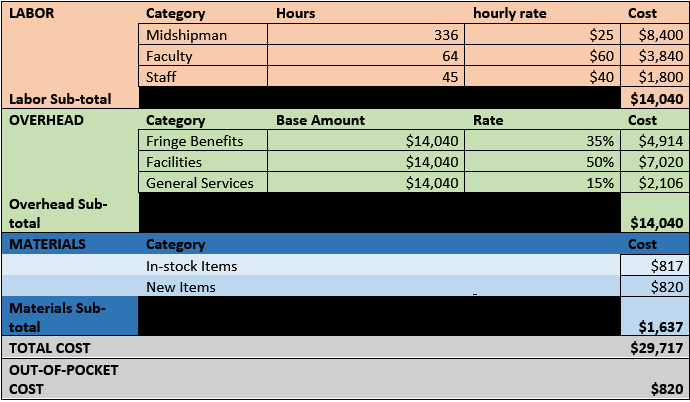
\includegraphics[width=0.8\columnwidth]{\myroot/figures/BUDGET_ew495report.png}
%\end{center}
%\label{table-budget}
%%just insert the table here as a figure... saved as a png
%\end{table}
%
%
%I have purchased and recieved all items that cover the originally proposed \$570 new item cost with the exception of a second additional Crazyflie 2.1 that was originally budgeted for, but I have not requested it yet for my research as I don't predict I will need it considering I have four old Crazyflie 2.0 models to use in addtion to the new 2.1 model I obtained with research funds. The increase in the total out-of-pocket cost is due to an approximately \SI{50}{\percent} increase added on to my original anticipated budget to account for any last-minute must-haves such as a battery charger that can charge multiple Crazyflies at once (will become more applicable as I get into more hardware testing). The in-stock item cost is derived from an approximated worth of \$198 for each of the four Crazyflie 2.0's that I'm using, as well as an additional \$25 for the use of old OptiTrack markers and the 3D printed rotor-guards.